\documentclass[mathserif]{beamer}
\usepackage[utf8]{inputenc}
\def\magyarOptions{defaults=hu-min}
\usepackage[magyar]{babel}
\usepackage{ifpdf}
\ifpdf
	\usepackage{epstopdf}
\fi
\usepackage{amsmath,amssymb}
\usepackage{faktor}
\usetheme{Boadilla}
\usecolortheme{default}
\usefonttheme{structurebold}
\beamertemplatenavigationsymbolsempty
\hypersetup{pdfpagemode=FullScreen}

\DeclareMathOperator{\Sym}{Sym}
\begin{document}

\title[Csoportelméleti Algoritmusok]{Csoportelméleti Algoritmusok}
\author{Nagy Gergely Gábor}
\institute{ELTE TTK}
\date{2012. január 20.}

\begin{frame}
\titlepage
\end{frame}

\begin{frame}{Vázlat}
\begin{itemize}
\item Véges csoportok számítógépes prezentációja
	\begin{itemize}
	\item Black-box csoportok
	\item Permutációcsoportok
	\item Véges test feletti mátrixcsoportok
	\item Policiklikus prezentáció (csak feloldható csoportokra)
	\end{itemize}
\item Karaktertáblázat számolása
	\begin{itemize}
	\item Burnside-Dixon-Schneider
	\item Conlon, Unger
	\end{itemize}
\item Wolfram Mathematica
\end{itemize}
\end{frame}

\begin{frame}{Black-box csoportok}
\begin{itemize}
\item $\Sigma$ ábécé feletti szavak az elemek
\item Egy szóról orákulummal el tudjuk dönteni, hogy egységelem-e
\item Inverzet, szorzatot tudunk számolni
\item Semmit nem tételezünk fel a csoport szerkezetéről
\item Pl: $G$ hat $\Omega$-n, $\omega^G$ orbitot meghatározhatjuk
\end{itemize}
\end{frame}

\begin{frame}{Permutációcsoportok}
\begin{itemize}
\item $\langle S \rangle = G \le \Sym(\Omega)$
\item Naív módszer a csoport tárolására: Felírjuk az összes csoportelemet
\item Legyen $B = (\beta_1, \dots, \beta_m)$ különböző $\Omega$-beli elemek sorozata.
\item Legyen $1\le i\le m+1$-re $G^{[i]} = G_{(\beta_1,\dots,\beta_{i-1})} = G_{\beta_1}\cap\dots\cap G_{\beta_{i-1}}$.
\item $B$ irredundáns bázis, ha $G^{[m+1]}=1$ és minden $G^{[i]}$ különböző.
\item Az $S$ generátorrendszer erős, ha minden $i$-re $\langle S \cap G^{[i]}\rangle = G^{[i]}$
\item Schreier-Sims algoritmussal tudunk erős generátorrendszert adni
\end{itemize}
\end{frame}

\begin{frame}{Permutációcsoportok}
\begin{itemize}
\item $\mathcal{P}$ tulajdonság, $G(\mathcal{P})$-t keressük
\item Mélységi bejárással kereshetünk elemeket
\item Báziselemek képeinek sorra történő meghatározásával
\item $\mathcal{P}$-től függően sokféle optimalizáció lehetséges
\item Gyakran $G(\mathcal{P})$ egy részcsoport vagy egy mellékosztály
\item Pl: $a,b\in G$ rögzítettekre $g \in G(\mathcal{P})$, ha $b = a^g = g^{-1}ag$\\
Erre $G(\mathcal{P})$ $C_G(a)$ mellékosztálya
\end{itemize}
\end{frame}

\begin{frame}{Konjugáltosztályok meghatározása}
\begin{itemize}
\item Osztályok reprezentánsait szeretnénk megtalálni
\item Lehet véletlen elemek próbálgatásával
\item Hátrány: kis konjugáltosztályt nagyon lassan találnánk meg
\item Jerrum (1995): Vegyük a véletlen elemet az utolsó centralizátorából!\\
Markov-láncokkal belátható, hogy így gyorsan megtaláljuk az összes osztályt
\end{itemize}
\end{frame}

\begin{frame}{Karaktertáblázat számolása}
\begin{itemize}
\item Legyenek $C_1, \dots, C_s$ a konjugáltosztályok ($C_1 = \{1\}$), $g_i \in C_i$, $h_i = |C_i|$.
\item $c_{jkl} = \left|\left\{(a,b)\in C_j \times C_k \mid ab = g_l\right\}\right|$. $M_j$ mátrix $(k,l)$-edik eleme $c_{jkl}$.
\item Irreducibilis karakterek $\chi^1, \dots, \chi^s$; $\chi^i_j = \chi^i(g_j)$; $d_i = \chi^i_1 = \chi^i(1)$.
\item $\forall i,j$ $(\chi^i_1,\dots,\chi^i_s)$ baloldali sajátvektora $M_j$-nek
\item Ezek a vektorok lineárisan függetlenek, így numberikusan megtalálhatóak konstansszorzó erejéig
\item $1 = \langle \chi^i, \chi^i \rangle = \frac{1}{|G|}\sum_{j=1}^s h_j |\chi^i_j|^2$ alapján a konstans is meghatározható
\end{itemize}
\end{frame}

\begin{frame}{Karaktertáblázat számolása}
\begin{itemize}
\item $e$ a csoport exponense, $\zeta$ komplex $e$-edik egységgyök
\item $\chi^i_j$-k algebrai egészek, sőt $\chi^i_j \in \mathbb{Z}[\zeta]$
\item Elvárható, hogy ne csak közelítő eredményt kapjunk
\item Dixon: $\mathbb{F}_p$ véges test felett számoljunk, végén vissza lehet kapni a komplex alakot
\item Schneider: nem szükséges az összes $M_j$ mátrix kiszámolása, csak bizonyos oszlopok kellenek
\end{itemize}
\end{frame}

\begin{frame}{Wolfram Mathematica példa}
\begin{itemize}
\item $D_8$ karaktertáblája:
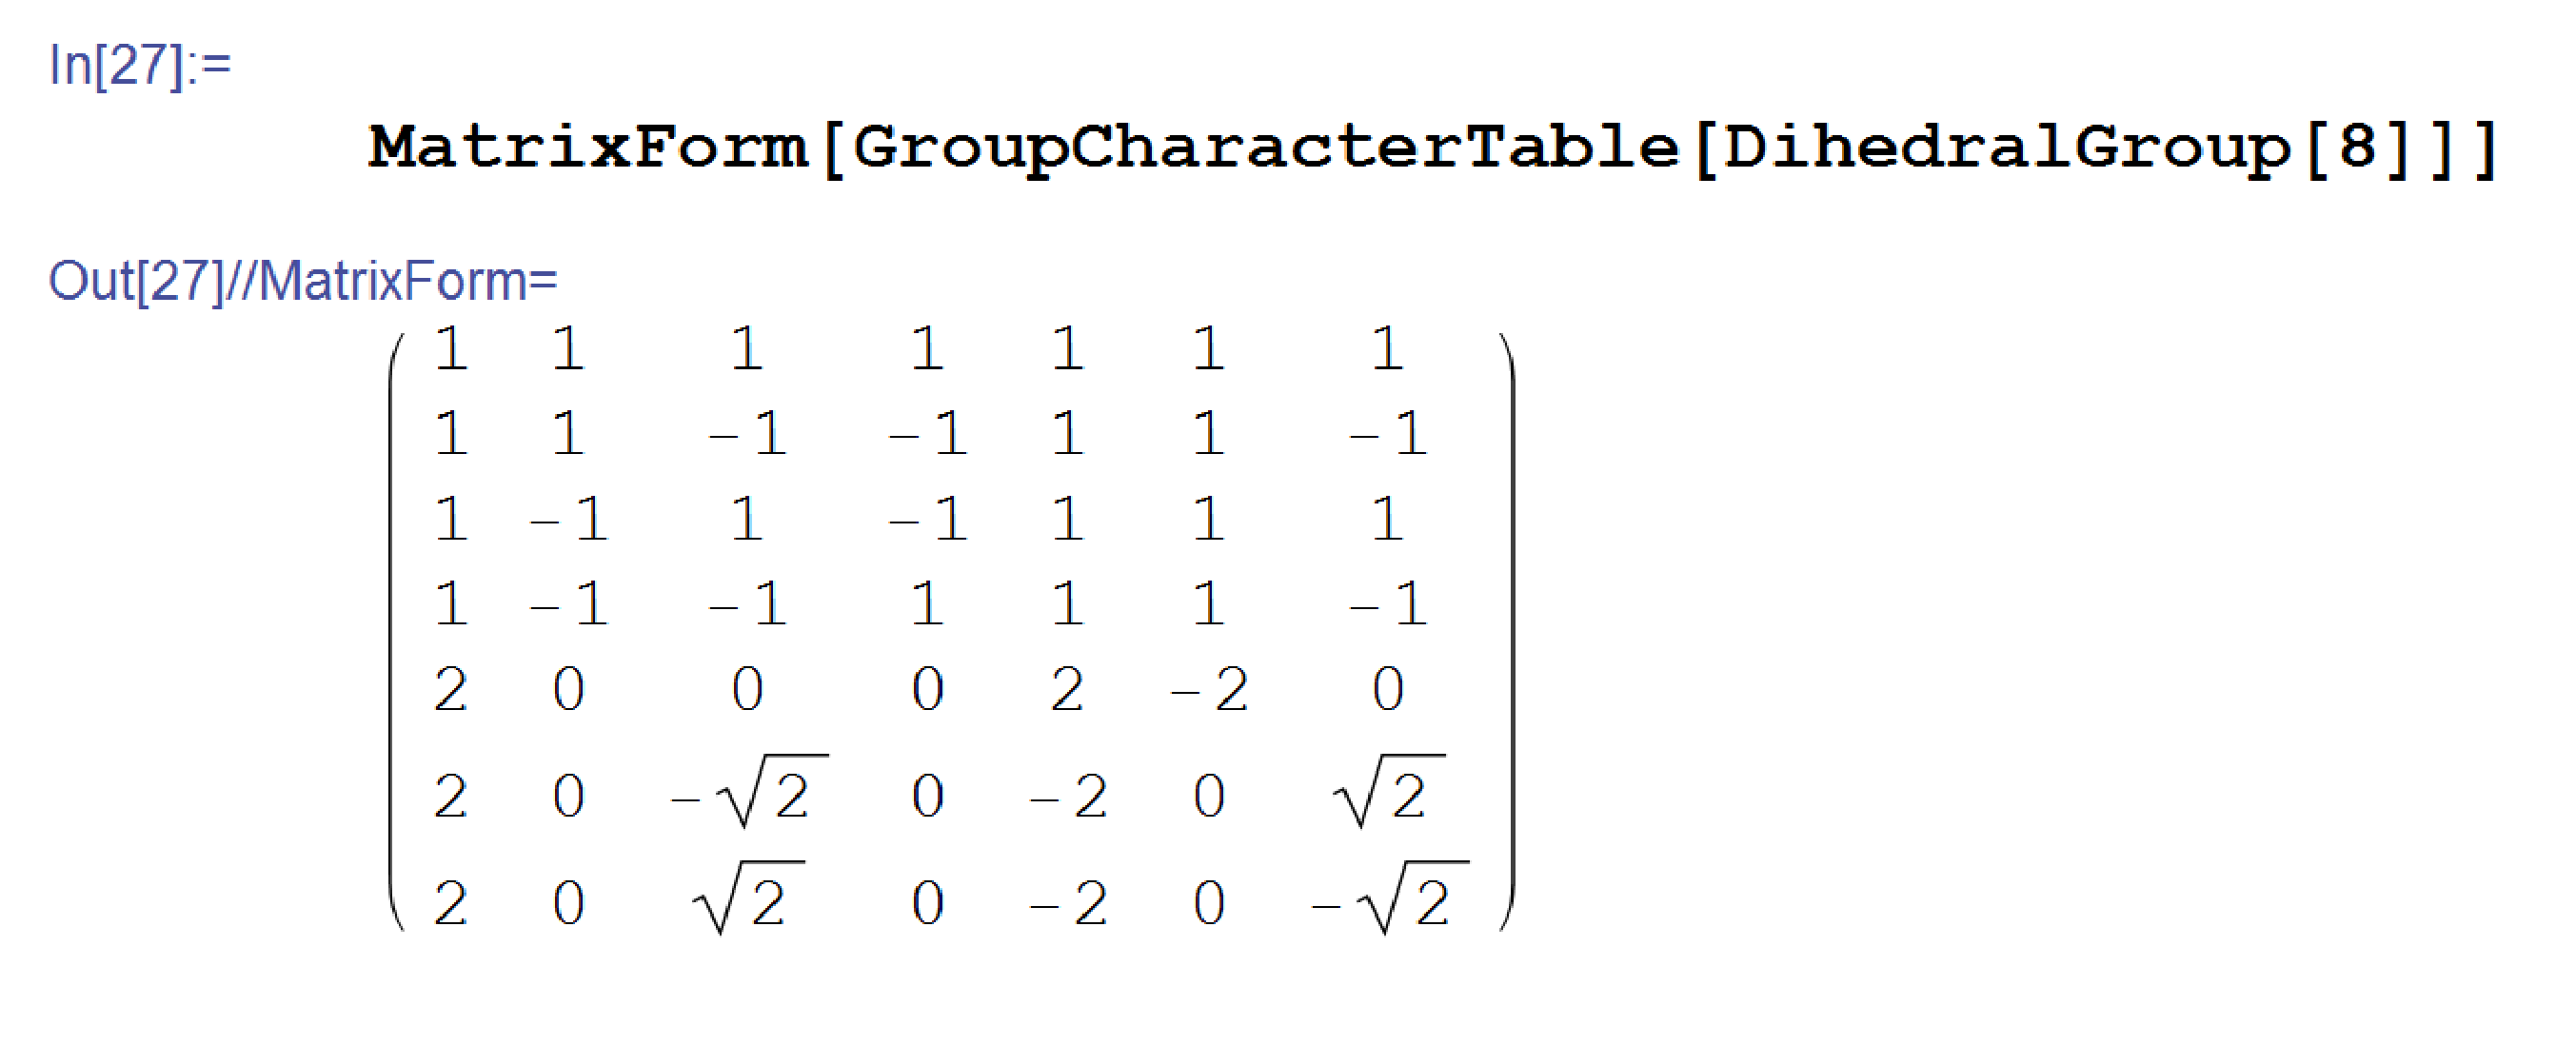
\includegraphics[scale=0.25]{d8}
\end{itemize}
\end{frame}

\begin{frame}{Wolfram Mathematica példa}
\begin{itemize}
\item $Z_2\times Z_4$ karaktertáblája:
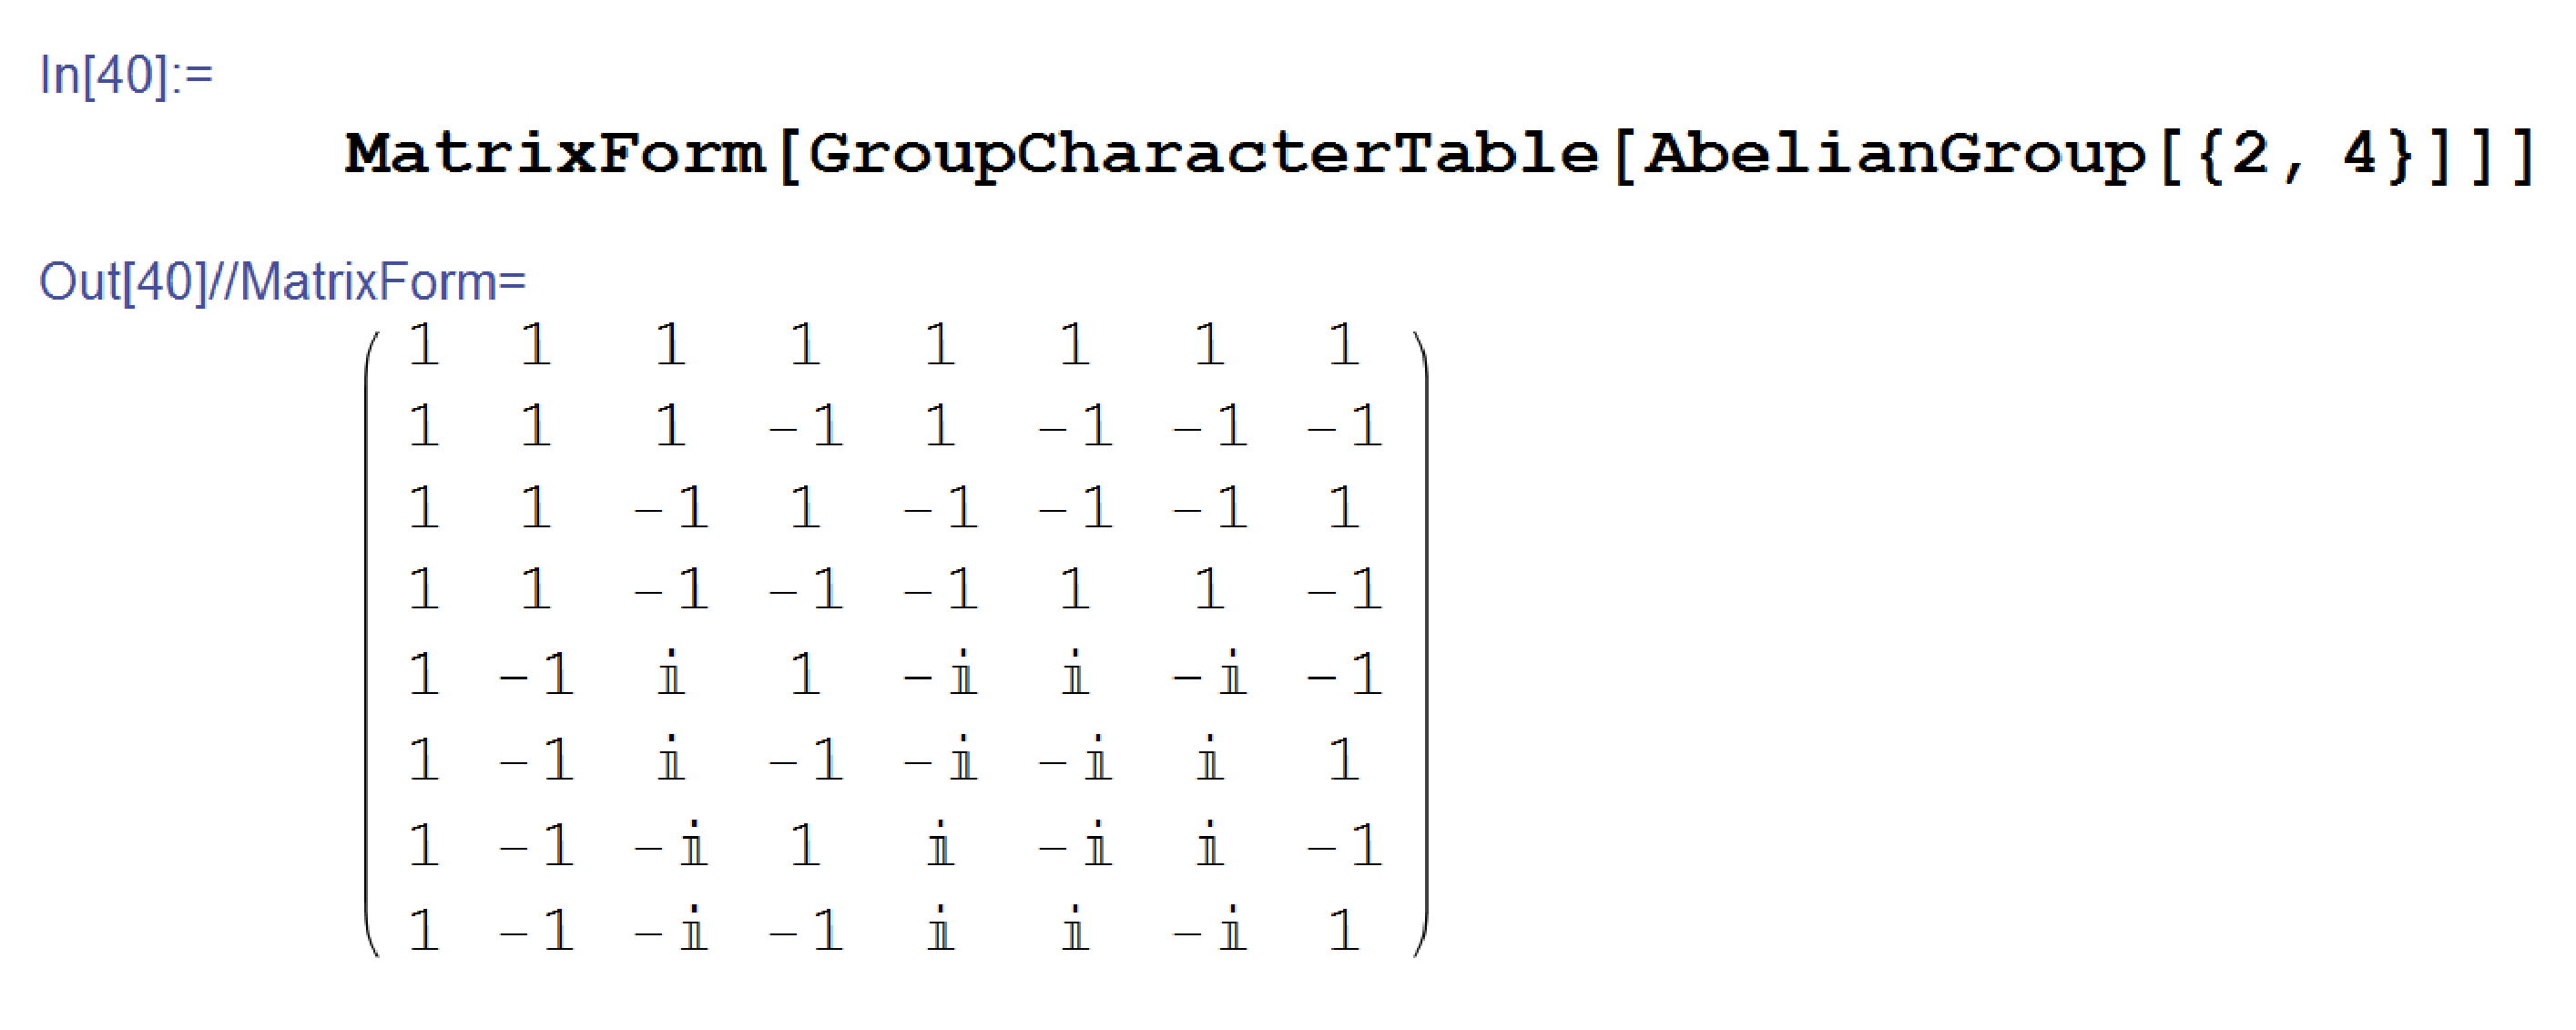
\includegraphics[scale=0.25]{z2z4}
\end{itemize}
\end{frame}

\begin{frame}{}
\hfill\huge{Köszönöm a figyelmet!}\hfill\hfill
\end{frame}

\end{document}
